\setcounter{page}{1}
\section*{Zielsetzung}
In dem Versuch $V408$ soll die Brennweite unterschiedlicher Linsen und
Linsensysteme untersucht werden.
\section{Theorie}
Die geometrische Optik ist nur gültig unter der Annahme, dass die Wellenlänge klein
gegenüber der Apperaturabmessung ist. Das Licht wird nicht als Welle, sondern als
Strahl betrachtet.  %Klingt so als ob die geometrische Optik von Linsen abhängig ist. Schreib lieber unter welchen Bedingungen die geom. Optik Gültigkeit hat.
Eine Linse besitzt im Vergleich zum Umgebungsmedium einen anderen Brechungsindex $n$.
Das bedeutet, dass das Licht nach dem Brechungsgesetz
\begin{equation*}
  n_1\sin(\alpha)=n_2\sin(\beta)
\end{equation*}
beim Erreichen und Verlassen der Linse gebrochen wird. %Erreichen, Verlassen

Linsen können weiter in \emph{Sammellinsen} und \emph{Zerstreuungslinsen} %nicht eine Linse, Zerstreuungslinsen
eingeteilt werden. Als Sammellinse werden die Linsen bezeichnet, die zum Linsenrand %man
dünner werden (vgl. Abbildung \ref{fig: sammellinse}) und dadurch das Licht in einem Punkt, als \emph{Brennpunkt} $f$ bezeichnet,
bündelt.
Bei einer Sammellinse sind Brennpunkt (\emph{Brennweite}) %-alias
und Bildweite $b$ (Abstand des Bildes zur Linse) positiv und es ergibt sich ein
\emph{reelles} Bild. Ein Bild wird genau dann als reell bezeichnet, wenn
ein Schirm es sichtbar macht.
Hingegen wird eine Zerstreuungslinse nach außen hin dicker (vgl. Abb. \ref{fig: zerstreungslinse}) und
defokusiert das Licht. Desweiteren sind Bildweite und Brennweite negativ.
Bei beiden Linsentypen werden Bild- und Gegenstandweite immer von der Mittelebene
aus angegeben.

Dem ist bei \emph{dicken Linsen} (vgl. Abb. \ref{fig: dicke_linse}) nicht so.
Bei diesen werden zwei Hauptebenen ($H$ und $H'$) eingeführt. Der einlaufende Strahl
wird nun gedanklich an jeder Hauptebene gebrochen.
\begin{figure}
  \centering
  \begin{subfigure}{0.48\textwidth}
    \centering
    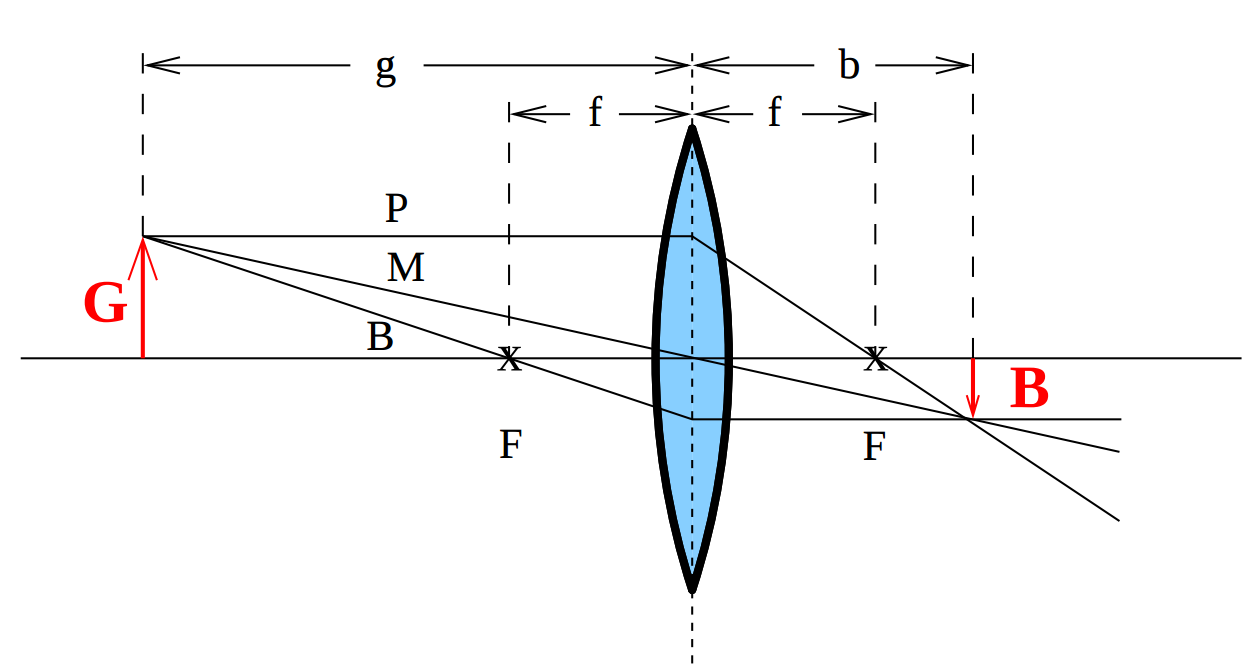
\includegraphics[width=1 \textwidth]{./pics/sammellinse.png}
    \caption{Sammellinse \cite{anleitung408}.}
    \label{fig: sammellinse}
  \end{subfigure}
  \begin{subfigure}{0.48\textwidth}
    \centering
    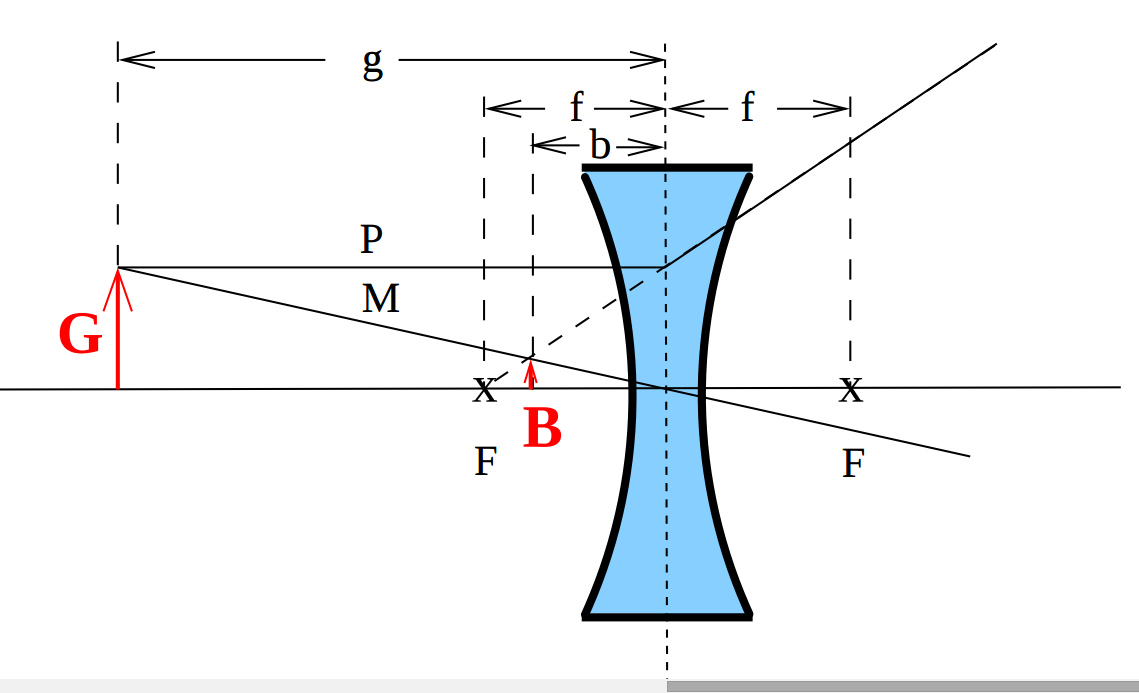
\includegraphics[width=1\textwidth]{./pics/zerstreungslinse.png}
    \caption{Zerstreuungslinse \cite{anleitung408}.}
    \label{fig: zerstreungslinse}
  \end{subfigure}
  \caption{Linsentypen}
  \label{fig: linsentypen}
\end{figure}
\begin{figure}
    \centering
    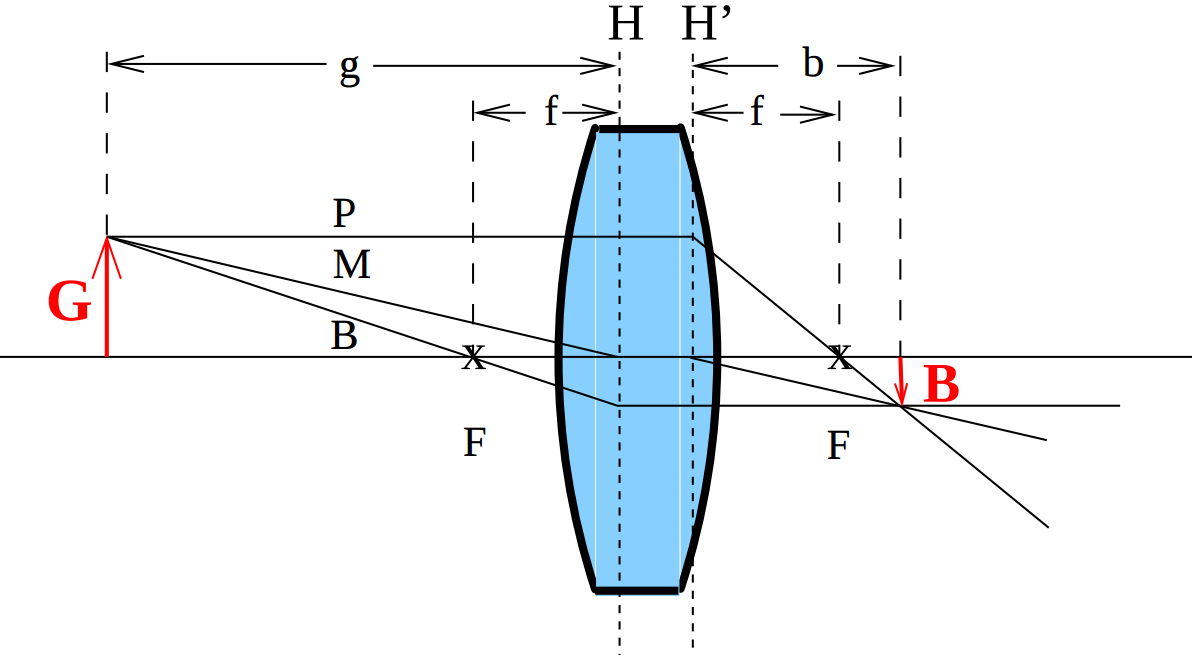
\includegraphics[width=0.6\textwidth]{./pics/dicke_linse.png}
    \caption{Dicke Linse \cite{anleitung408}.}
    \label{fig: dicke_linse}
\end{figure}

Um den Bildpunkt einer Linse zu konstruieren, werden drei Strahlen benötigt.
Zu diesen gehört der Parallelstrahl $P$, der Mittelpunktstrahl $M$ und der
Brennpunktstrahl $B$.
Der Parallelstrahl verläuft parallel zur optischen Achse und wird in der Hauptebene
zum Brennpunkt gebrochen. Der Mittelpunktstrahl verläuft vom Gegenstand mittig durch die
Linse. Zunächst läuft der Brennpunktstrahl durch den Brennpunkt der Linse, wird dann
an der Hauptebene gebrochen und verläuft dann parallel zur optischen Achse.
Aus der Bildkonstruktion folgt das \emph{Abbildungsgesetz} %man
\begin{align}
  \label{eq: abbildungsgesetz_gross}
  V_1=\frac{B}{G}=\frac{b}{g}
\end{align}
Hierbei beschreibt $V$ den Abbildungsmaßstab, $B$ die Bildgröße, Bildweite $b$, $G$ die Gegenstandsgröße
und $g$ die Gegenstandsweite. %was ist mit b?

Aus Gleichung \eqref{eq: abbildungsgesetz_gross} bzw. \eqref{eq: abbildungsgesetz_klein}
kann die Linsengleichung für dünne Linsen abgeleitet werden:
\begin{equation}
  \label{eq: linsengleichung}
  \frac{1}{f}= \frac{1}{b}+  \frac{1}{g} \qquad \Leftrightarrow \quad f= \frac{gb}{g+b}.
\end{equation}

Wie oben erwähnt werden bei dicken Linsen zwei Hauptebenen verwendet, um das Brechverhalten
zu beschreiben. Dieses Verfahren wird zusätzlich auch bei Linsensystemen (vgl. Abbildung \ref{fig: linsensystem}) verwendet. %wird, systemen
Um die Brennweite eines Linsensystems (hier bestehend aus zwei Linsen) zu bestimmen, kann folgende Gleichung verwendet werden:
\begin{equation}
  \label{eq: gleichung_linsensystem}
  \frac{1}{f}=\frac{1}{f_1}+\frac{1}{f_2}-\frac{d}{f_1f_2}.
\end{equation}
Hierbei seien $f_1 \, \text{und} \, f_2$ die Brennweiten der beiden Linsen und $d$ der
Abstand der beiden Hauptebenen.
Die Bild-, Brenn- und Gegenstandsweite werden dann zur jeweiligen Hauptebene
bestimmt und sichern so die Gültigkeit der Linsengleichung.
Dennoch bietet das Hauptebensystem keine ideale Lösung, denn streng genommen
gilt es nur für achsennahe Strahlen. Bei achsenfernen Strahlen wird das Licht stärker
gebrochen und es können \emph{Abbildungsfehler}, z.\,B. nicht mehr scharfes Abbilden eines Bildes,
auftreten. Solche Fehler treten bei \emph{spährischer} und \emph{chromatischen} Abberration auf.
Bei der sphärischen Abberration liegt der Brennweite von achsenfernen Strahlen näher zur
Mittelebene als bei achsennahen Strahlen.
Ist die Lichtbrechung Abhängig von der Frequenz,
wird von der chromatische Abberration gesprochen.
Der Brennpunkt von blauem Licht liegt näher an der Mittelebene, als %wellenlängenabhängige, klingt unschön
bei rotem Licht. In der Optik wird dieses als Dispersion bezeichnet.
 %man

Eine weitere wichtige optische Größe ist die \emph{Brechkraft}
\begin{equation}
  \label{eq: brechkraft}
  D=\frac{1}{f}
\end{equation}
mit der Einheit Dioptrie $\map{dpt}=\si{\per \meter}$.
Bei einem Linsensystem, bestehend aus mehreren dünnen Linsen, die gesamte %man
Brechkraft $D\ua{G}$ ergibt sich aus Summation der einzelnen Brechkräfte %Brecchkräft
\begin{equation*}
  D\ua{G}=\sum_{i=1}^{N}D_i \qquad N\in\mathbb{N}.
\end{equation*}
Unter der Bedingung das zwischen den beiden Linsen kein Abstand exestiert.
